\documentclass[10pt]{article}

\usepackage[margin=0.62in,headheight=13pt]{geometry}
\usepackage[T1]{fontenc}
\usepackage{lmodern}
\usepackage{amsmath,amssymb}
\usepackage{xcolor}
\usepackage{booktabs}
\usepackage{tabularx}
\usepackage{array}
\usepackage{tikz}
\usepackage{needspace}
\usepackage{algpseudocode}
\usepackage{fancyhdr}
\usepackage[hidelinks]{hyperref}

\definecolor{headc}{HTML}{1F3864}
\definecolor{barc}{HTML}{FBE3D6}
\definecolor{newc}{HTML}{2E7D32}
\definecolor{tgtc}{HTML}{C62828}

\setlength{\parindent}{0pt}
\setlength{\parskip}{0.22em plus 0.05em minus 0.05em}
\setlength{\tabcolsep}{3.5pt}
\newcolumntype{Y}{>{\raggedright\arraybackslash}X}

\pagestyle{fancy}
\fancyhf{}
\fancyhead[L]{\scriptsize EECE 7205 \textbar\ BST In-Class Work}
\fancyhead[R]{\scriptsize MyungJin Suh}
\fancyfoot[C]{\scriptsize\thepage}
\renewcommand{\headrulewidth}{0.3pt}

\hypersetup{pdftitle={EECE 7205 BST In-Class Work},pdfauthor={MyungJin Suh}}

\algrenewcommand\algorithmicrequire{\textbf{Input:}}
\algrenewcommand\algorithmicensure{\textbf{Output:}}
\newenvironment{algo}[2]{%
  \par\needspace{5\baselineskip}\noindent{\small\textbf{#1}\quad\textnormal{#2}}\par\nopagebreak
  \vspace{-0.35em}\footnotesize\begin{algorithmic}[1]
}{\end{algorithmic}\par}
\newenvironment{mini}{\par\vspace{-0.15em}\footnotesize\begin{algorithmic}[1]}{\end{algorithmic}\vspace{-0.25em}}

\tikzset{
  bnode/.style={circle, draw, line width=0.6pt, fill=white, minimum size=5.4mm, inner sep=0pt, font=\scriptsize},
  see/.style={bnode, draw=headc, line width=1.15pt},
  hit/.style={bnode, fill=headc, text=white, draw=headc, line width=0.8pt},
  cut/.style={bnode, draw=tgtc, line width=1.2pt},
  nil/.style={circle, draw=headc, dashed, line width=0.7pt, fill=white, minimum size=5mm, inner sep=0pt, font=\tiny},
  btree/.style={
    baseline=(current bounding box.north),
    level distance=8.6mm,
    level 1/.style={sibling distance=28mm},
    level 2/.style={sibling distance=15mm},
    level 3/.style={sibling distance=9mm},
    level 4/.style={sibling distance=9mm},
    edge from parent/.style={draw, line width=0.55pt}
  },
  /bst/k20/.style={bnode}, /bst/k30/.style={bnode}, /bst/k35/.style={bnode},
  /bst/k40/.style={bnode}, /bst/k45/.style={bnode}, /bst/k50/.style={bnode},
  /bst/k60/.style={bnode}, /bst/k65/.style={bnode}, /bst/k70/.style={bnode},
  /bst/k75/.style={bnode}, /bst/k80/.style={bnode}
}
\newcommand{\clearmarks}{\tikzset{
  /bst/k20/.style={bnode}, /bst/k30/.style={bnode}, /bst/k35/.style={bnode},
  /bst/k40/.style={bnode}, /bst/k45/.style={bnode}, /bst/k50/.style={bnode},
  /bst/k60/.style={bnode}, /bst/k65/.style={bnode}, /bst/k70/.style={bnode},
  /bst/k75/.style={bnode}, /bst/k80/.style={bnode}
}}

\newcommand{\treeFinal}{%
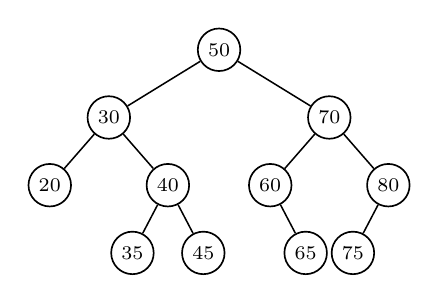
\begin{tikzpicture}[btree]
\node[/bst/k50] {50}
  child { node[/bst/k30] {30}
    child { node[/bst/k20] {20} }
    child { node[/bst/k40] {40}
      child { node[/bst/k35] {35} }
      child { node[/bst/k45] {45} }
    }
  }
  child { node[/bst/k70] {70}
    child { node[/bst/k60] {60}
      child[missing] {}
      child { node[/bst/k65] {65} }
    }
    child { node[/bst/k80] {80}
      child { node[/bst/k75] {75} }
      child[missing] {}
    }
  };
\end{tikzpicture}\clearmarks}

\newcommand{\treeNilThirtyThree}{%
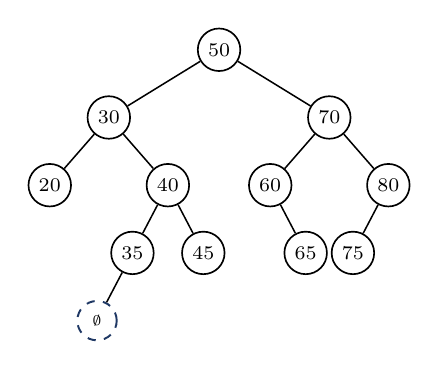
\begin{tikzpicture}[btree]
\node[/bst/k50] {50}
  child { node[/bst/k30] {30}
    child { node[/bst/k20] {20} }
    child { node[/bst/k40] {40}
      child { node[/bst/k35] {35}
        child { node[nil] {$\emptyset$} }
        child[missing] {}
      }
      child { node[/bst/k45] {45} }
    }
  }
  child { node[/bst/k70] {70}
    child { node[/bst/k60] {60}
      child[missing] {}
      child { node[/bst/k65] {65} }
    }
    child { node[/bst/k80] {80}
      child { node[/bst/k75] {75} }
      child[missing] {}
    }
  };
\end{tikzpicture}\clearmarks}

\newcommand{\treeNilNinety}{%
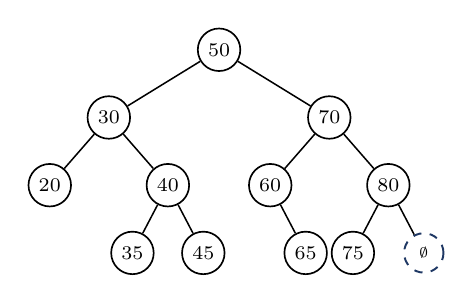
\begin{tikzpicture}[btree]
\node[/bst/k50] {50}
  child { node[/bst/k30] {30}
    child { node[/bst/k20] {20} }
    child { node[/bst/k40] {40}
      child { node[/bst/k35] {35} }
      child { node[/bst/k45] {45} }
    }
  }
  child { node[/bst/k70] {70}
    child { node[/bst/k60] {60}
      child[missing] {}
      child { node[/bst/k65] {65} }
    }
    child { node[/bst/k80] {80}
      child { node[/bst/k75] {75} }
      child { node[nil] {$\emptyset$} }
    }
  };
\end{tikzpicture}\clearmarks}

\newcommand{\sw}[2]{\tikz[baseline=-0.55ex]\node[#1, minimum size=3.3mm, inner sep=0pt] at (0,0) {};\,\textcolor{black}{#2}}

\newcommand{\prob}[1]{%
  \par\needspace{6\baselineskip}\vspace{4pt}%
  {\large\bfseries\color{headc}#1}\par\vspace{0pt}%
  \noindent\textcolor{headc}{\rule{\linewidth}{0.6pt}}\par\vspace{1pt}}

\newcommand{\casehead}[2]{%
  \par\vspace{3pt}\needspace{16mm}%
  \noindent\colorbox{barc}{\parbox{\dimexpr\linewidth-2\fboxsep}{\bfseries\color{headc}#1%
    \if\relax\detokenize{#2}\relax\else\hfill{\mdseries Rules: #2}\fi}}\par\vspace{1pt}}

\newcommand{\pair}[4]{%
  \par\smallskip\noindent
  \begin{minipage}[t]{0.49\linewidth}\centering
    {\footnotesize\bfseries #1}\\[3pt]#2
  \end{minipage}\hfill
  \begin{minipage}[t]{0.49\linewidth}\centering
    {\footnotesize\bfseries #3}\\[3pt]#4
  \end{minipage}\par\smallskip}

\newcommand{\onepic}[2]{%
  \par\smallskip\noindent
  \begin{minipage}{\linewidth}\centering
    {\footnotesize\bfseries #1}\\[3pt]#2
  \end{minipage}\par\smallskip}

\begin{document}

\begin{center}
{\Large\bfseries\color{headc} Binary Search Trees}\\[1pt]
{\normalsize In-Class Work}\\[1pt]
EECE 7205: Fundamentals of Computer Engineering \quad Fall 2026\\
MyungJin Suh \quad October 22, 2026
\end{center}

\vspace{-0.4em}
\noindent Same array in every problem:
$\textit{arr}=\{50,30,70,20,40,60,80,35,45,65,75\}$, $n=11$.
A new insert is always a leaf. Height of an empty tree is $-1$, so one node has height $0$.
\hfill
\sw{hit}{added / found / rewritten}
\quad\sw{see}{compared}
\quad\sw{cut}{deleted}
\quad\sw{nil}{NULL}

\prob{Problem 1. Insert}

\casehead{Case 1. Insert 50 into an empty tree}{I1}
\texttt{root} is NULL, so 50 becomes the root. No comparison.
\pair{Before}{\footnotesize\textit{(empty)}}{After}{%

\begin{tikzpicture}[btree]\node[hit]{50};\end{tikzpicture}}

\casehead{Case 2. Insert 30}{I2, I1}
$30<50$, and the left child of 50 is NULL. Attach 30 there. 1 comparison.
\begin{mini}
\If{key $<$ cur.key}
  \If{cur.left $=$ NULL}
    \State cur.left $\gets$ newNode \Comment{I1}
    \State \Return
  \EndIf
  \State cur $\gets$ cur.left \Comment{I2}
\EndIf
\end{mini}
\pair{Before}{
\begin{tikzpicture}[btree]\node[see]{50};\end{tikzpicture}}{After}{%
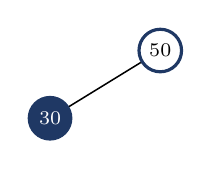
\begin{tikzpicture}[btree]
\node[see]{50} child { node[hit]{30} } child[missing] {};
\end{tikzpicture}}

\casehead{Case 3. Insert 70}{I3, I1}
$70>50$, and the right child of 50 is NULL. Attach 70 there. 1 comparison.
\begin{mini}
\If{key $>$ cur.key}
  \If{cur.right $=$ NULL}
    \State cur.right $\gets$ newNode \Comment{I1}
    \State \Return
  \EndIf
  \State cur $\gets$ cur.right \Comment{I3}
\EndIf
\end{mini}
\pair{Before}{%
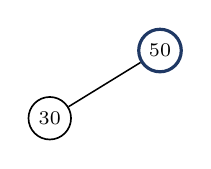
\begin{tikzpicture}[btree]
\node[see]{50} child { node[bnode]{30} } child[missing] {};
\end{tikzpicture}}{After}{%
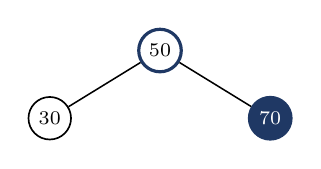
\begin{tikzpicture}[btree]
\node[see]{50} child { node[bnode]{30} } child { node[hit]{70} };
\end{tikzpicture}}

\casehead{Case 4. Insert 20, 40, 60, 80, then 35}{I2 / I3, then I1}
\begin{center}
\footnotesize
\begin{tabular}{@{}clll@{}}
\toprule
Key & Compared & Rules & Attached as \\
\midrule
20 & 50, 30 & I2, I2, I1 & left of 30 \\
40 & 50, 30 & I2, I3, I1 & right of 30 \\
60 & 50, 70 & I3, I2, I1 & left of 70 \\
80 & 50, 70 & I3, I3, I1 & right of 70 \\
35 & 50, 30, 40 & I2, I3, I2, I1 & left of 40 \\
\bottomrule
\end{tabular}
\end{center}
35 goes left at 50 because $35<50$, and right at 30 because $35>30$. The side is the comparison with the current node. 3 comparisons.
\begin{mini}
\Loop
  \If{key $<$ cur.key}
    \If{cur.left $=$ NULL}
      \State cur.left $\gets$ newNode; \textbf{return} \Comment{I1}
    \EndIf
    \State cur $\gets$ cur.left \Comment{I2}
  \ElsIf{key $>$ cur.key}
    \If{cur.right $=$ NULL}
      \State cur.right $\gets$ newNode; \textbf{return} \Comment{I1}
    \EndIf
    \State cur $\gets$ cur.right \Comment{I3}
  \EndIf
\EndLoop
\end{mini}
\pair{Before 35}{%
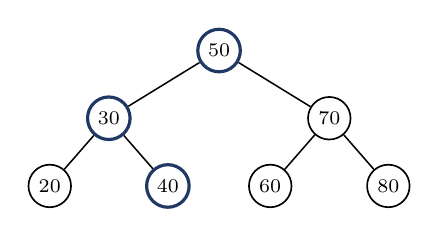
\begin{tikzpicture}[btree]
\node[see]{50}
  child { node[see]{30}
    child { node[bnode]{20} }
    child { node[see]{40} } }
  child { node[bnode]{70}
    child { node[bnode]{60} }
    child { node[bnode]{80} } };
\end{tikzpicture}}{After: 35 left of 40}{%
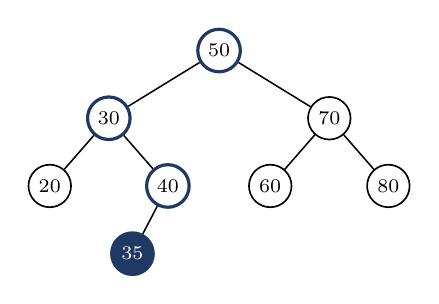
\begin{tikzpicture}[btree]
\node[see]{50}
  child { node[see]{30}
    child { node[bnode]{20} }
    child { node[see]{40}
      child { node[hit]{35} } child[missing] {} } }
  child { node[bnode]{70}
    child { node[bnode]{60} }
    child { node[bnode]{80} } };
\end{tikzpicture}}

\casehead{Case 5. Finish the tree, then insert 40 again}{I4}
45 compared with 50, 30, 40 (I2, I3, I3, I1): right of 40.
65 compared with 50, 70, 60 (I3, I2, I3, I1): right of 60.
75 compared with 50, 70, 80 (I3, I3, I2, I1): left of 80.
Height 3. Inorder $20\,30\,35\,40\,45\,50\,60\,65\,70\,75\,80$.
Inserting 40 again walks 50, 30, 40 and hits I4, so the tree is unchanged. An equal key is neither smaller nor larger, so it has no child slot. Keys stay distinct.
\begin{mini}
\If{key $=$ cur.key}
  \State \Return \Comment{I4}
\EndIf
\end{mini}
\onepic{Final tree. The second 40 stops on the marked path.}{%
\tikzset{/bst/k50/.style={see},/bst/k30/.style={see},/bst/k40/.style={hit}}\treeFinal}

\casehead{Case 6. Sorted keys 20, 30, 40, 50, 60}{I1, then I3 + I1}
20 is the root (I1). Every later key is larger than every key already stored, so each step is I3 and the right child is NULL (I1). Height $n-1=4$. The 11-key tree has height 3, so sorted input makes the taller tree.
\begin{algo}{BUILD-FROM-ARRAY(data, $n$)}{}
\For{$i \gets 0$ to $n-1$}
  \State INSERT(data[$i$])
\EndFor
\end{algo}
\pair{Before}{\footnotesize\textit{(empty)}}{Height 4}{%
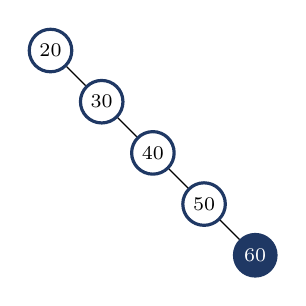
\begin{tikzpicture}[x=6.5mm,y=6.5mm,baseline=(current bounding box.north)]
  \node[see] (a) at (0,0) {20};
  \node[see] (b) at (1,-1) {30};
  \node[see] (c) at (2,-2) {40};
  \node[see] (d) at (3,-3) {50};
  \node[hit] (e) at (4,-4) {60};
  \draw (a)--(b) (b)--(c) (c)--(d) (d)--(e);
\end{tikzpicture}}

\casehead{(g) All 11 insertions}{}
\begin{center}
\footnotesize
\begin{tabular}{@{}clllll@{}}
\toprule
Step & Insert & Compared & Rules & Parent & Side \\
\midrule
1 & 50 & --- & I1 & --- & root \\
2 & 30 & 50 & I2, I1 & 50 & Left \\
3 & 70 & 50 & I3, I1 & 50 & Right \\
4 & 20 & 50, 30 & I2, I2, I1 & 30 & Left \\
5 & 40 & 50, 30 & I2, I3, I1 & 30 & Right \\
6 & 60 & 50, 70 & I3, I2, I1 & 70 & Left \\
7 & 80 & 50, 70 & I3, I3, I1 & 70 & Right \\
8 & 35 & 50, 30, 40 & I2, I3, I2, I1 & 40 & Left \\
9 & 45 & 50, 30, 40 & I2, I3, I3, I1 & 40 & Right \\
10 & 65 & 50, 70, 60 & I3, I2, I3, I1 & 60 & Right \\
11 & 75 & 50, 70, 80 & I3, I3, I2, I1 & 80 & Left \\
\bottomrule
\end{tabular}
\end{center}

\casehead{(h) INSERT, and the deepest insert}{I1--I4}
The deepest inserts are 35, 45, 65, and 75. Each compares with 3 nodes, equal to the height: the new leaf hangs at depth 3.
\begin{algo}{INSERT(key)}{}
\State \textit{newNode} $\gets$ a new node with key
\If{root $=$ NULL}
  \State root $\gets$ newNode; \textbf{return} \Comment{I1}
\EndIf
\State cur $\gets$ root
\Loop
  \If{key $<$ cur.key}
    \If{cur.left $=$ NULL}
      \State cur.left $\gets$ newNode; \textbf{return} \Comment{I1}
    \EndIf
    \State cur $\gets$ cur.left \Comment{I2}
  \ElsIf{key $>$ cur.key}
    \If{cur.right $=$ NULL}
      \State cur.right $\gets$ newNode; \textbf{return} \Comment{I1}
    \EndIf
    \State cur $\gets$ cur.right \Comment{I3}
  \Else
    \State \Return \Comment{I4}
  \EndIf
\EndLoop
\end{algo}

\prob{Problem 2. Search}

One path from the root. The comparison count is the number of keys compared. Reaching NULL is S1 and does not add a comparison.

\begin{algo}{SEARCH(target)}{used by every case}
\State cur $\gets$ root
\While{cur $\neq$ NULL}
  \If{target $=$ cur.key}
    \State \Return FOUND \Comment{S2}
  \ElsIf{target $<$ cur.key}
    \State cur $\gets$ cur.left \Comment{S3}
  \Else
    \State cur $\gets$ cur.right \Comment{S4}
  \EndIf
\EndWhile
\State \Return NOT FOUND \Comment{S1}
\end{algo}

\casehead{Case 1. Search 50}{S2}
$50=50$ at the root. 1 comparison.
\onepic{Path: 50}{\tikzset{/bst/k50/.style={hit}}\treeFinal}

\casehead{Case 2. Search 45}{S3, S4, S4, S2}
$45<50$ left, $45>30$ right, $45>40$ right, $45=45$. Path $50\to 30\to 40\to 45$. 4 comparisons. The right subtree of 50 is skipped.
\onepic{Path: $50\to 30\to 40\to 45$}{%
\tikzset{/bst/k50/.style={see},/bst/k30/.style={see},/bst/k40/.style={see},/bst/k45/.style={hit}}\treeFinal}

\casehead{Case 3. Search 65}{S4, S3, S4, S2}
$65>50$ right, $65<70$ left, $65>60$ right, $65=65$. Path $50\to 70\to 60\to 65$. 4 comparisons.
\onepic{Path: $50\to 70\to 60\to 65$}{%
\tikzset{/bst/k50/.style={see},/bst/k70/.style={see},/bst/k60/.style={see},/bst/k65/.style={hit}}\treeFinal}

\casehead{Case 4. Search 33}{S3, S4, S3, S3, S1}
$33<50$, $33>30$, $33<40$, $33<35$, then the left child of 35 is NULL. Path $50\to 30\to 40\to 35\to$ NULL. 4 comparisons. Inserting 33 would make it the left child of 35.
\onepic{Stops on the missing left child of 35}{%
\tikzset{/bst/k50/.style={see},/bst/k30/.style={see},/bst/k40/.style={see},/bst/k35/.style={see}}\treeNilThirtyThree}

\casehead{Case 5. Search 90}{S4, S4, S4, S1}
90 is greater than 50, 70, and 80, so the walk only goes right and falls off 80. Path $50\to 70\to 80\to$ NULL. 3 comparisons. Inserted, 90 would be the right child of 80.
\onepic{Stops on the missing right child of 80}{%
\tikzset{/bst/k50/.style={see},/bst/k70/.style={see},/bst/k80/.style={see}}\treeNilNinety}

\casehead{Case 6. Minimum and maximum}{P2}
No target. Minimum follows left children until the left pointer is NULL: $50\to 30\to 20$. Maximum follows right children: $50\to 70\to 80$.
\begin{mini}
\While{node.left $\neq$ NULL}
  \State node $\gets$ node.left
\EndWhile
\State \Return node.key \Comment{FIND-MIN: 20}
\While{node.right $\neq$ NULL}
  \State node $\gets$ node.right
\EndWhile
\State \Return node.key \Comment{FIND-MAX: 80, called from the root}
\end{mini}
\onepic{Left spine is the minimum. Right spine is the maximum.}{%
\tikzset{/bst/k50/.style={see},/bst/k30/.style={see},/bst/k20/.style={hit},/bst/k70/.style={see},/bst/k80/.style={hit}}\treeFinal}

\casehead{Search table}{}
\begin{center}
\footnotesize
\begin{tabularx}{\linewidth}{@{}c c Y l l c@{}}
\toprule
Case & Target & Nodes compared & Rules & Result & Comparisons \\
\midrule
1 & 50 & 50 & S2 & found & 1 \\
2 & 45 & 50, 30, 40, 45 & S3, S4, S4, S2 & found & 4 \\
3 & 65 & 50, 70, 60, 65 & S4, S3, S4, S2 & found & 4 \\
4 & 33 & 50, 30, 40, 35 & S3, S4, S3, S3, S1 & not found & 4 \\
5 & 90 & 50, 70, 80 & S4, S4, S4, S1 & not found & 3 \\
6 & min / max & 50, 30, 20 / 50, 70, 80 & P2 & 20 / 80 & 0 \\
\bottomrule
\end{tabularx}
\end{center}
\textbf{(g)} Longest search: 4 comparisons $= h+1$. A path has at most one node per level, and this tree has height 3.

\prob{Problem 3. Delete}

Each case starts again from the 11-key tree. Search first, then use the number of children.

\casehead{Case 1. Delete 33}{S1}
Same failed search as above: $50\to 30\to 40\to 35\to$ NULL. Nothing is removed.
\begin{mini}
\If{node $=$ NULL}
  \State \Return NULL \Comment{S1}
\EndIf
\end{mini}
\onepic{Unchanged}{%
\tikzset{/bst/k50/.style={see},/bst/k30/.style={see},/bst/k40/.style={see},/bst/k35/.style={see}}\treeNilThirtyThree}

\casehead{Case 2. Delete 20}{D1}
20 is a leaf. The left pointer of 30 becomes NULL.
\begin{mini}
\If{node.left $=$ NULL \textbf{and} node.right $=$ NULL}
  \State \Return NULL \Comment{D1}
\EndIf
\end{mini}
\pair{Before}{\tikzset{/bst/k20/.style={cut}}\treeFinal}{After}{%
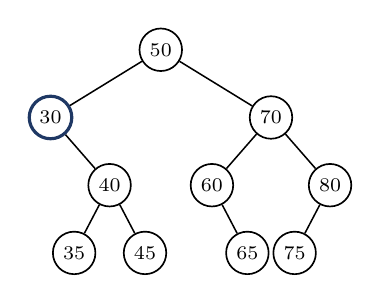
\begin{tikzpicture}[btree]
\node[bnode]{50}
  child { node[see]{30}
    child[missing] {}
    child { node[bnode]{40}
      child { node[bnode]{35} }
      child { node[bnode]{45} } } }
  child { node[bnode]{70}
    child { node[bnode]{60} child[missing] {} child { node[bnode]{65} } }
    child { node[bnode]{80} child { node[bnode]{75} } child[missing] {} } };
\end{tikzpicture}}

\casehead{Case 3. Delete 60}{D2}
60 has only a right child, 65. \texttt{70.left} now points at 65.
\begin{mini}
\If{node.left $=$ NULL}
  \State \Return node.right \Comment{D2}
\EndIf
\end{mini}
\pair{Before}{\tikzset{/bst/k60/.style={cut}}\treeFinal}{After}{%
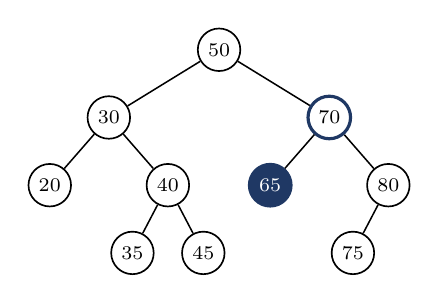
\begin{tikzpicture}[btree]
\node[bnode]{50}
  child { node[bnode]{30}
    child { node[bnode]{20} }
    child { node[bnode]{40}
      child { node[bnode]{35} } child { node[bnode]{45} } } }
  child { node[see]{70}
    child { node[hit]{65} }
    child { node[bnode]{80} child { node[bnode]{75} } child[missing] {} } };
\end{tikzpicture}}

\casehead{Case 4. Delete 80}{D2}
80 has only a left child, 75. \texttt{70.right} now points at 75.
\begin{mini}
\If{node.right $=$ NULL}
  \State \Return node.left \Comment{D2}
\EndIf
\end{mini}
\pair{Before}{\tikzset{/bst/k80/.style={cut}}\treeFinal}{After}{%
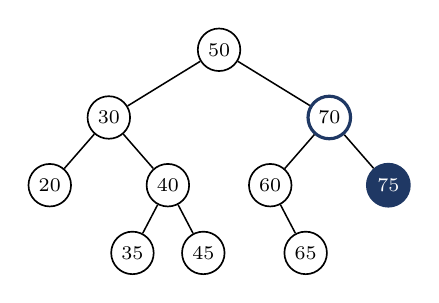
\begin{tikzpicture}[btree]
\node[bnode]{50}
  child { node[bnode]{30}
    child { node[bnode]{20} }
    child { node[bnode]{40}
      child { node[bnode]{35} } child { node[bnode]{45} } } }
  child { node[see]{70}
    child { node[bnode]{60} child[missing] {} child { node[bnode]{65} } }
    child { node[hit]{75} } };
\end{tikzpicture}}

\casehead{Case 5. Delete 40}{D3, then D1}
40 has two children, so D3. Successor: go right once. 45 has no left child, so the successor is 40's own right child. Copy 45 into the node, then delete 45. That node is a leaf, so the second step is D1.
\begin{mini}
\State $s \gets$ node.right \Comment{45, and $s$.left is NULL}
\State node.key $\gets s$.key
\State node.right $\gets$ DELETE(node.right, $s$.key) \Comment{D1}
\end{mini}
\pair{Before}{\tikzset{/bst/k40/.style={cut},/bst/k45/.style={see}}\treeFinal}{After}{%
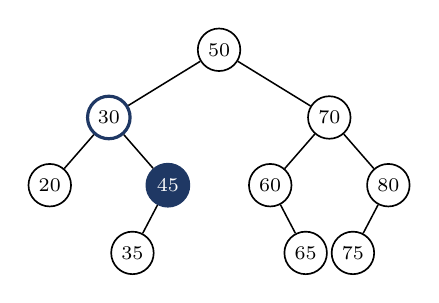
\begin{tikzpicture}[btree]
\node[bnode]{50}
  child { node[see]{30}
    child { node[bnode]{20} }
    child { node[hit]{45}
      child { node[bnode]{35} } child[missing] {} } }
  child { node[bnode]{70}
    child { node[bnode]{60} child[missing] {} child { node[bnode]{65} } }
    child { node[bnode]{80} child { node[bnode]{75} } child[missing] {} } };
\end{tikzpicture}}

\casehead{Case 6. Delete 50}{D3, then D2}
50 has two children. Successor: right to 70, then left to 60. Copy 60 into the root. The old 60 has a right child, 65, and no left child, so deleting it is D2: \texttt{70.left} points at 65. A successor has no left child, so removing it is D1 or D2.
\begin{mini}
\State $s \gets$ node.right \Comment{70}
\While{$s$.left $\neq$ NULL}
  \State $s \gets s$.left \Comment{60}
\EndWhile
\State node.key $\gets s$.key
\State node.right $\gets$ DELETE(node.right, $s$.key) \Comment{D2, returns 65}
\end{mini}
\pair{Before}{%
\tikzset{/bst/k50/.style={cut},/bst/k70/.style={see},/bst/k60/.style={see}}\treeFinal}{After}{%
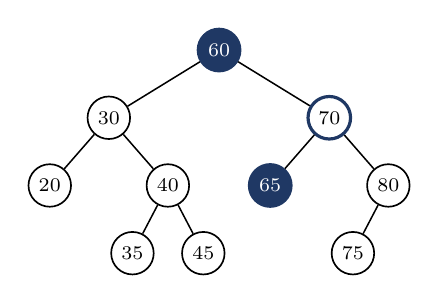
\begin{tikzpicture}[btree]
\node[hit]{60}
  child { node[bnode]{30}
    child { node[bnode]{20} }
    child { node[bnode]{40}
      child { node[bnode]{35} } child { node[bnode]{45} } } }
  child { node[see]{70}
    child { node[hit]{65} }
    child { node[bnode]{80} child { node[bnode]{75} } child[missing] {} } };
\end{tikzpicture}}

\casehead{Delete table}{}
\footnotesize
\begin{tabularx}{\linewidth}{@{}c c Y c l Y@{}}
\toprule
Case & Delete & Children & Successor & Rules & Level order after \\
\midrule
1 & 33 & not found & --- & S1 & 50 30 70 20 40 60 80 35 45 65 75 \\
2 & 20 & none & --- & D1 & 50 30 70 40 60 80 35 45 65 75 \\
3 & 60 & right: 65 & --- & D2 & 50 30 70 20 40 65 80 35 45 75 \\
4 & 80 & left: 75 & --- & D2 & 50 30 70 20 40 60 75 35 45 65 \\
5 & 40 & 35 and 45 & 45 & D3, D1 & 50 30 70 20 45 60 80 35 65 75 \\
6 & 50 & 30 and 70 & 60 & D3, D2 & 60 30 70 20 40 65 80 35 45 75 \\
\bottomrule
\end{tabularx}

\casehead{(g) DELETE}{S1, D1, D2, D3}
\begin{algo}{DELETE(node, key)}{returns the new subtree root}
\If{node $=$ NULL}
  \State \Return NULL \Comment{S1}
\EndIf
\If{key $<$ node.key}
  \State node.left $\gets$ DELETE(node.left, key)
\ElsIf{key $>$ node.key}
  \State node.right $\gets$ DELETE(node.right, key)
\Else
  \If{node.left $=$ NULL}
    \State \Return node.right \Comment{D1, or D2}
  \EndIf
  \If{node.right $=$ NULL}
    \State \Return node.left \Comment{D2}
  \EndIf
  \State $s \gets$ node.right
  \While{$s$.left $\neq$ NULL}
    \State $s \gets s$.left \Comment{successor}
  \EndWhile
  \State node.key $\gets s$.key
  \State node.right $\gets$ DELETE(node.right, $s$.key)
\EndIf
\State \Return node
\end{algo}

\casehead{(h) Why the inorder successor}{}
The successor is the next key in sorted order: the smallest key in the right subtree. It is larger than everything on the left and smaller than everything else on the right, so copying it keeps the BST property. It has no left child, so removing it is D1 or D2. The deepest node can be any key, and putting it in the hole can break that order.

\end{document}
